\documentclass[a4paper,12pt]{report}
\usepackage[utf8]{vietnam}
\usepackage{graphicx}
\usepackage{geometry}
\usepackage{fancyhdr}
\usepackage{titlesec}
\usepackage{indentfirst}
\usepackage{adjustbox}
\usepackage{float}
\usepackage{listings}
\usepackage{tcolorbox}
\usepackage{xcolor}
\usepackage{amsmath} 
\usepackage{tikz}
\usepackage{xcolor}
\usepackage{algorithm}
\usepackage{algpseudocode}
% \usepackage[utf8]{inputenc}
% \usepackage[T1]{fontenc}

% Canh lề rộng hơn một chút cho đẹp
\geometry{
  top=2.5cm,
  bottom=2.5cm,
  left=2.5cm,
  right=2.5cm
}
\lstset{
  language=C++,
  basicstyle=\ttfamily\small,
  breaklines=true,
  showstringspaces=false,
  commentstyle=\color{gray},
  frame=none
}

\begin{document}

\begin{center}
    {\bfseries\LARGE ĐẠI HỌC BÁCH KHOA HÀ NỘI}\\[0.5em]
    {\Large Trường Công nghệ Thông tin và Truyền thông}\\[2em]

    % Logo SOICT lớn hơn
    \includegraphics[width=12cm]{images/logo_soict.png}\\[3em]

    {\Huge\bfseries BÀI TẬP LỚN}\\[1em]
    {\Large\bfseries NHẬP MÔN TRÍ TUỆ NHÂN TẠO}\\[1em]
    {\Large  Hệ Thống AI Dự Đoán Bệnh Tiểu Đường Sử Dụng Thuật Toán KNN tối ưu bằng PSO và Naive Bayes}\\[4em]

    \begin{table}[h!]
    \centering
    \begin{tabular}{l @{\hspace{2cm}} l}
    \textbf{Họ và Tên} & \textbf{Mã số sinh viên} \\
    Nguyễn Việt Dũng     &    20235688 \\
    Hoàng Đức Anh      &    20235640 \\
    Nguyễn Nhật Minh     &     20235781 \\
    Đỗ Khắc Hoàng     &     20235721 \\
    \end{tabular}
    \end{table}

    \begin{center}
    \textbf{Giảng viên hướng dẫn:} TS. Đỗ Tiến Dũng
    \end{center}

    \vfill
    {\normalsize Hà Nội, tháng 06 năm 2026}
\end{center}
%trang 2 

\newpage

\tableofcontents
\newpage

\chapter{Giới thiệu chung}

\section{Đặt vấn đề}

Trong bối cảnh y tế số hiện đại, tiểu đường (Diabetes Mellitus) đang là một trong những thách thức sức khỏe cộng đồng lớn nhất toàn cầu. Việc phát hiện và chẩn đoán sớm bệnh lý này đóng vai trò sống còn trong việc ngăn chặn các biến chứng nghiêm trọng. Với sự phát triển của Trí tuệ Nhân tạo (AI) và Học máy (Machine Learning), các hệ thống hỗ trợ quyết định y khoa dựa trên dữ liệu sinh học đang trở thành công cụ đắc lực cho bác sĩ. Tuy nhiên, việc xây dựng một mô hình dự đoán chính xác và ổn định từ dữ liệu y tế (như bộ dữ liệu Pima Indians Diabetes) vẫn đối mặt với nhiều rào cản kỹ thuật:

\begin{enumerate}
    \item \textbf{Đặc thù phức tạp của dữ liệu y tế:} 
    Dữ liệu sinh học thường chứa nhiều nhiễu, có sự mất cân bằng giữa các lớp (class imbalance) và sự chênh lệch lớn về thang đo giữa các đặc trưng (ví dụ: Nồng độ Insulin so với số lần mang thai). Việc sử dụng toàn bộ 8 chỉ số y tế để huấn luyện có thể dẫn đến hiện tượng "lời nguyền số chiều" (curse of dimensionality), trong đó các đặc trưng không quan trọng làm mờ nhạt đi thông tin của các đặc trưng cốt lõi.

    \item \textbf{Hạn chế của các thuật toán phân loại cơ bản:} 
    \begin{itemize}
        \item Thuật toán \textbf{K-Nearest Neighbors (KNN)} có ưu điểm trực quan và linh hoạt, nhưng hiệu suất lại phụ thuộc quá lớn vào siêu tham số $k$ và đặc biệt nhạy cảm với dữ liệu nhiễu. Nếu không có cơ chế chọn lọc, KNN truyền thống sẽ tính toán khoảng cách dựa trên cả những đặc trưng kém quan trọng, làm giảm sút nghiêm trọng độ chính xác.
        \item Thuật toán \textbf{Naive Bayes} cung cấp tốc độ tính toán nhanh dựa trên lý thuyết xác suất, nhưng lại mang giả định các đặc trưng là hoàn toàn độc lập (feature independence) – một điều kiện rất hiếm khi thỏa mãn hoàn toàn trong thực tế y khoa.
    \end{itemize}

    \item \textbf{Bài toán lựa chọn đặc trưng (Feature Selection) và tinh chỉnh tham số:} 
    Để khắc phục điểm yếu của KNN, hệ thống cần một cơ chế tự động hóa để loại bỏ các đặc trưng nhiễu, giữ lại tập đặc trưng tối ưu nhất và tìm ra giá trị $k$ lý tưởng. Đây là một bài toán tối ưu hóa tổ hợp rời rạc với không gian tìm kiếm rộng $\left(2^8 \times \text{khoảng giá trị của } k\right)$.
\end{enumerate}

\textbf{Kết luận:} 
Từ những thách thức trên, đề tài \textit{"Hệ Thống AI Dự Đoán Bệnh Tiểu Đường Sử Dụng Thuật Toán KNN tối ưu bằng PSO và Naive Bayes"} được đề xuất. Cốt lõi của giải pháp là ứng dụng thuật toán \textbf{Tối ưu hóa Bầy đàn dạng nhị phân (Binary PSO - BPSO)} để thực hiện quá trình Lựa chọn đặc trưng (Feature Selection) và tinh chỉnh tham số $k$ cho mô hình KNN. Đồng thời, mô hình Naive Bayes được sử dụng song song để đánh giá chéo và thiết lập cơ sở tham chiếu (baseline), qua đó xây dựng một hệ thống chẩn đoán bệnh tiểu đường toàn diện, đạt độ tin cậy và độ chính xác cao.

\newpage

\section{Giải pháp và Mục tiêu}

Để giải quyết các vấn đề cốt lõi đã đặt ra trong việc chẩn đoán bệnh tiểu đường, các giải pháp kỹ thuật và mục tiêu cụ thể được đề xuất như sau:

\subsection*{1. Giải pháp đề xuất: Mô hình lai KNN-BPSO và Naive Bayes}
Hệ thống được thiết kế dựa trên sự kết hợp giữa kỹ thuật tối ưu hóa siêu heuristic không gian rời rạc và các thuật toán học máy thống kê:
\begin{itemize}
    \item \textbf{Lựa chọn đặc trưng và tối ưu siêu tham số bằng Binary PSO (BPSO):} 
    Thuật toán Tối ưu hóa Bầy đàn dạng nhị phân (BPSO) được sử dụng để giải quyết bài toán lựa chọn đặc trưng. Trong không gian tìm kiếm, mỗi "hạt" (particle) đại diện cho một bộ cấu hình bao gồm: một vector nhị phân chiều dài 8 (tương ứng với 8 chỉ số sinh học, trong đó bit $1$ nghĩa là đặc trưng được giữ lại, bit $0$ là loại bỏ) và giá trị $k$ của KNN. BPSO sẽ liên tục cập nhật vị trí các hạt thông qua hàm mục tiêu (Fitness Function) nhằm cân bằng giữa việc tối đa hóa độ chính xác phân loại và tối thiểu hóa số lượng đặc trưng đầu vào.
    
    \item \textbf{Phân loại bằng K-Nearest Neighbors (KNN) trên không gian giảm chiều:} 
    Thay vì tính toán trên toàn bộ 8 đặc trưng nguyên thủy, mô hình KNN chỉ thực hiện tính toán khoảng cách và phân loại dựa trên tập con các đặc trưng đã được BPSO chọn lọc. Cơ chế này giúp loại bỏ triệt để các thông tin nhiễu, thu gọn không gian dữ liệu, từ đó cải thiện đáng kể cả tốc độ tính toán lẫn độ chính xác của hệ thống dự đoán.
    
    \item \textbf{Đối sánh độc lập với Naive Bayes:} 
    Thuật toán Naive Bayes được triển khai độc lập để tạo ra một cơ sở tham chiếu vững chắc. Bằng cách so sánh hiệu năng giữa thuật toán xác suất cổ điển này với giải pháp lai KNN-BPSO, báo cáo sẽ làm nổi bật tính ưu việt của phương pháp lựa chọn đặc trưng tối ưu trong việc xử lý các tập dữ liệu y tế phức tạp.
\end{itemize}

\subsection*{2. Mục tiêu nghiên cứu cụ thể}
Việc thực hiện đề tài hướng tới hoàn thành các mục tiêu khoa học và thực tiễn sau:
\begin{itemize}
    \item \textbf{Nâng cao hiệu suất dự đoán:} Cải thiện các chỉ số đánh giá cốt lõi (Accuracy, F1-Score, Sensitivity/Recall) trên bộ dữ liệu Pima Indians Diabetes so với việc chạy KNN trên toàn bộ 8 đặc trưng gốc.
    \item \textbf{Tự động hóa trích xuất đặc trưng:} Xây dựng thành công quy trình BPSO để tự động sàng lọc và xác định được tập hợp các chỉ số y tế thực sự có ý nghĩa quyết định đối với bệnh tiểu đường, giảm thiểu s\chapter{Mô hình phân lớp K-Nearest Neighbors}

\section{Lý thuyết thuật toán K-Nearest Neighbors}
Thuật toán K-Nearest Neighbors (KNN) là một phương pháp học máy giám sát phi tham số (non-parametric) hoạt động dựa trên nguyên lý lười (lazy learning). Không giống như các thuật toán xây dựng một mô hình toán học tổng quát từ dữ liệu huấn luyện (như hồi quy tuyến tính hay mạng nơ-ron), KNN lưu trữ toàn bộ các mẫu huấn luyện trong bộ nhớ và chỉ thực hiện tính toán khi có truy vấn dự đoán cho một mẫu dữ liệu mới.

\subsection{Nguyên lý hoạt động}
Cho một tập dữ liệu huấn luyện $T = \{(x_1, y_1), (x_2, y_2), \dots, (x_N, y_N)\}$ gồm $N$ mẫu, trong đó $x_i \in \mathbb{R}^d$ là vector đặc trưng $d$ chiều và $y_i$ là nhãn lớp tương ứng. Khi nhận được một mẫu kiểm thử cần dự đoán $q \in \mathbb{R}^d$, thuật toán KNN thực hiện các bước sau:
\begin{enumerate}
    \item \textbf{Tính khoảng cách:} Tính toán khoảng cách giữa mẫu truy vấn $q$ và tất cả các mẫu $x_i$ trong tập huấn luyện.
    \item \textbf{Tìm lân cận gần nhất:} Sắp xếp các khoảng cách tăng dần để chọn ra tập hợp $N_k(q)$ chứa $k$ mẫu huấn luyện có khoảng cách gần $q$ nhất.
    \item \textbf{Bỏ phiếu quyết định (Majority Voting):} Xác định lớp $\hat{y}$ cho mẫu $q$ bằng phương pháp lấy đa số phiếu bầu từ nhãn của $k$ lân cận:
    \begin{equation}
        \hat{y} = \arg\max_{c} \sum_{x_i \in N_k(q)} \mathbb{I}(y_i = c)
    \end{equation}
    Trong đó $\mathbb{I}(\cdot)$ là hàm chỉ thị (indicator function), nhận giá trị bằng $1$ nếu biểu thức bên trong đúng và bằng $0$ nếu biểu thức sai.
\end{enumerate}

\subsection{Các độ đo khoảng cách}
Độ chính xác của thuật toán KNN phụ thuộc rất lớn vào việc lựa chọn độ đo khoảng cách phù hợp để phản ánh chính xác sự tương đồng giữa hai mẫu dữ liệu $x = (x_1, x_2, \dots, x_d)$ và $q = (q_1, q_2, \dots, q_d)$:
\begin{itemize}
    \item \textbf{Khoảng cách Euclidean:} Đo khoảng cách theo đường thẳng trực tiếp trong không gian Euclid:
    \begin{equation}
        d_{\text{Euclidean}}(x, q) = \sqrt{\sum_{j=1}^{d} (x_j - q_j)^2}
    \end{equation}
    \item \textbf{Khoảng cách Manhattan:} Tổng khoảng cách theo chiều ngang và dọc dọc theo các trục tọa độ vuông góc:
    \begin{equation}
        d_{\text{Manhattan}}(x, q) = \sum_{j=1}^{d} |x_j - q_j|
    \end{equation}
\end{itemize}

\subsection{Cơ chế giải quyết xung đột nhãn (Tie-breaking)}
Khi số lượng lân cận $k$ là một số chẵn hoặc bài toán phân loại đa lớp, có khả năng xuất hiện sự hòa phiếu giữa hai hay nhiều nhãn lớp (ví dụ: $k=4$, 2 lân cận thuộc lớp A và 2 lân cận thuộc lớp B). Để giải quyết tình huống này, cài đặt của chúng tôi áp dụng cơ chế tie-breaking dựa trên thứ tự nhãn lớp: lớp có giá trị chỉ số lớp nhỏ nhất (nhãn có thứ tự nhỏ nhất) sẽ được chọn làm nhãn dự đoán cuối cùng.

\section{Phân tích dữ liệu và Tiền xử lý}
Trong nghiên cứu này, bộ dữ liệu \textbf{Pima Indians Diabetes} được sử dụng để dự đoán khả năng mắc bệnh tiểu đường ở bệnh nhân. Dữ liệu ban đầu gồm $768$ bệnh nhân với $8$ thuộc tính y tế làm đặc trưng đầu vào và thuộc tính mục tiêu \texttt{Outcome}.

\subsection{Khảo sát và Thống kê Đặc trưng}
Thống kê ban đầu về khoảng giá trị của $8$ thuộc tính được thể hiện ở Bảng~\ref{tab:feature_ranges}:

\begin{table}[H]
\centering
\caption{Khoảng giá trị của các đặc trưng ban đầu}
\label{tab:feature_ranges}
\begin{tabular}{lrrr}
\toprule
\textbf{Tên đặc trưng} & \textbf{Giá trị nhỏ nhất} & \textbf{Giá trị lớn nhất} & \textbf{Khoảng biến thiên} \\
\midrule
Pregnancies & 0.00 & 17.00 & 17.00 \\
Glucose & 0.00 & 199.00 & 199.00 \\
BloodPressure & 0.00 & 122.00 & 122.00 \\
SkinThickness & 0.00 & 99.00 & 99.00 \\
Insulin & 0.00 & 846.00 & 846.00 \\
BMI & 0.00 & 67.10 & 67.10 \\
DiabetesPedigreeFunction & 0.08 & 2.42 & 2.34 \\
Age & 21.00 & 81.00 & 60.00 \\
\bottomrule
\end{tabular}
\end{table}

\subsection{Phát hiện và xử lý ngoại lai bằng IQR}
Như được minh họa trên Hình~\ref{fig:boxplot_before}, dữ liệu gốc chứa rất nhiều điểm ngoại lai (outliers) ở tất cả các thuộc tính đặc trưng. Để loại bỏ các giá trị nhiễu này, chúng tôi áp dụng phương pháp khoảng trải giữa (Interquartile Range - IQR):
\begin{equation}
    \text{IQR} = Q_3 - Q_1
\end{equation}
Ngưỡng biên để xác định dữ liệu bình thường là:
\begin{equation}
    [\text{Biên dưới}, \text{Biên trên}] = [Q_1 - 1.5 \times \text{IQR}, Q_3 + 1.5 \times \text{IQR}]
\end{equation}
Trong đó $Q_1$ là phân vị thứ $25$ và $Q_3$ là phân vị thứ $75$. Các mẫu nằm ngoài ngưỡng này được xác định là dữ liệu nhiễu ngoại lai và bị loại bỏ khỏi tập dữ liệu.

\begin{figure}[H]
    \centering
    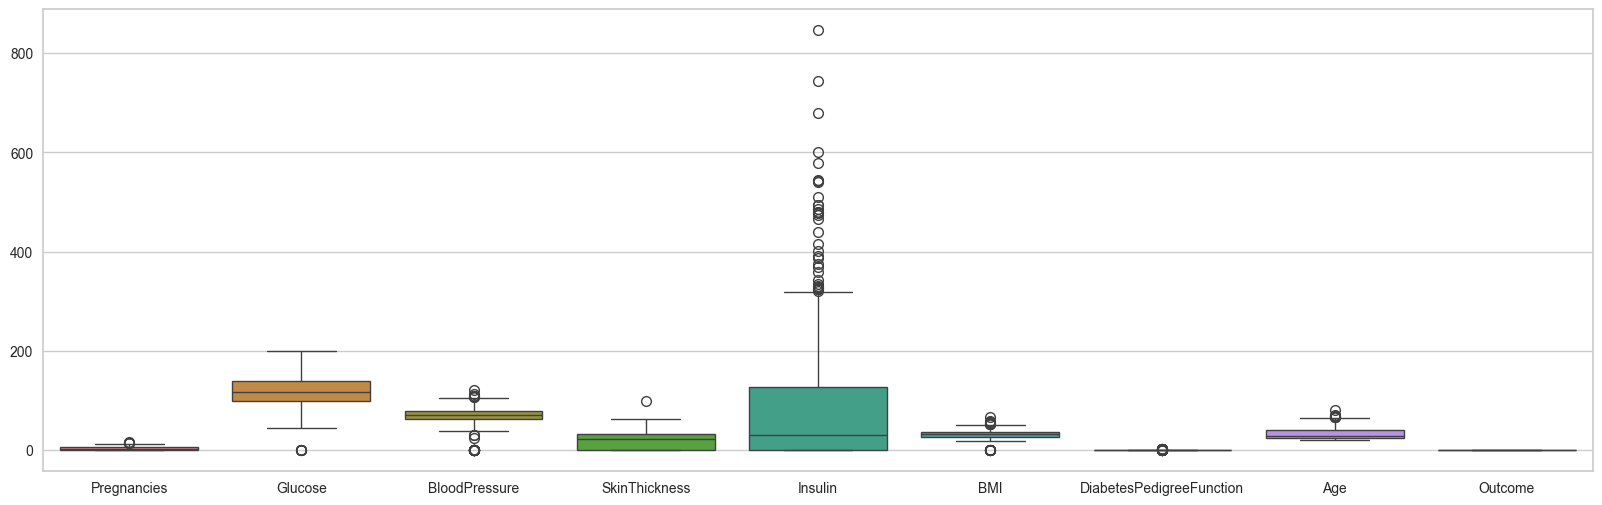
\includegraphics[width=0.9\textwidth]{images/boxplot_before_outliers.png}
    \caption{Biểu đồ Boxplot phân bố dữ liệu ban đầu}
    \label{fig:boxplot_before}
\end{figure}

Sau bước xử lý ngoại lai, kích thước tập dữ liệu giảm từ $768$ mẫu xuống còn $639$ mẫu sạch. Sự thay đổi trong phân bố đặc trưng sau khi loại bỏ ngoại lai được minh họa trong Hình~\ref{fig:boxplot_after}.

\begin{figure}[H]
    \centering
    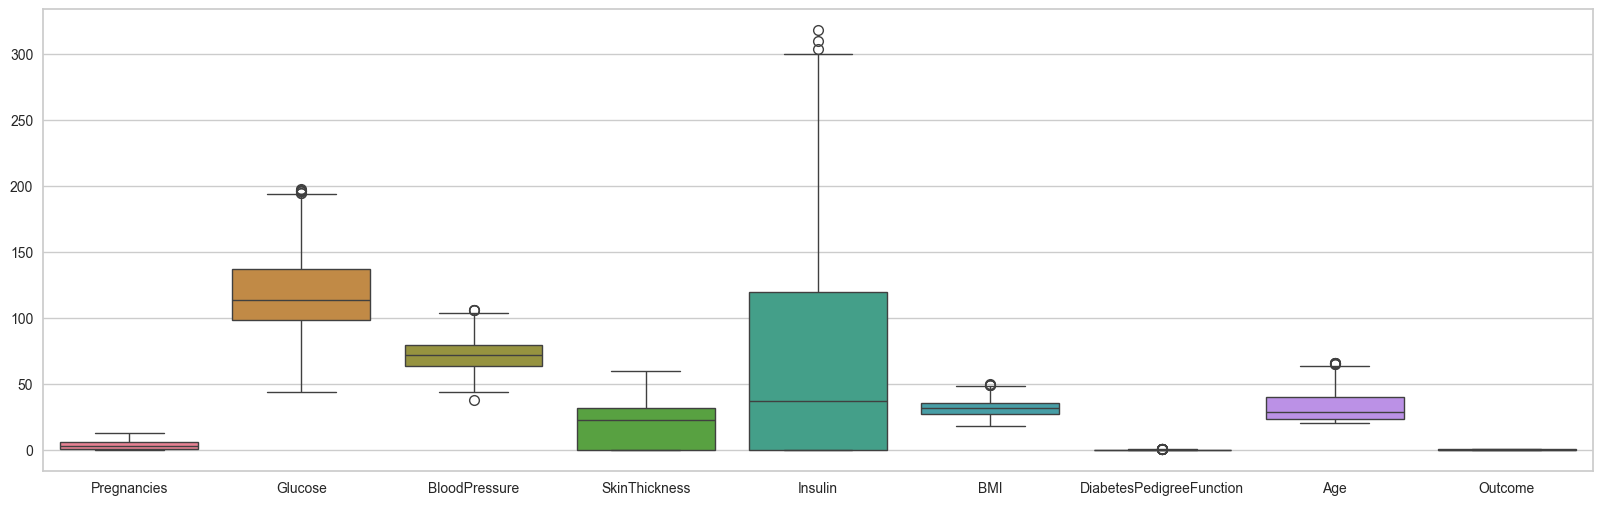
\includegraphics[width=0.9\textwidth]{images/boxplot_after_outliers.png}
    \caption{Biểu đồ Boxplot phân bố dữ liệu sau khi loại bỏ ngoại lai}
    \label{fig:boxplot_after}
\end{figure}

\subsection{Phân phối nhãn mục tiêu và Tương quan đặc trưng}
Trong tập dữ liệu ban đầu, phân phối của nhãn mục tiêu \texttt{Outcome} mất cân bằng tương đối với $500$ bệnh nhân khỏe mạnh (nhãn $0$) và $268$ bệnh nhân mắc bệnh tiểu đường (nhãn $1$), như được thể hiện ở Hình~\ref{fig:outcome_dist}.

\begin{figure}[H]
    \centering
    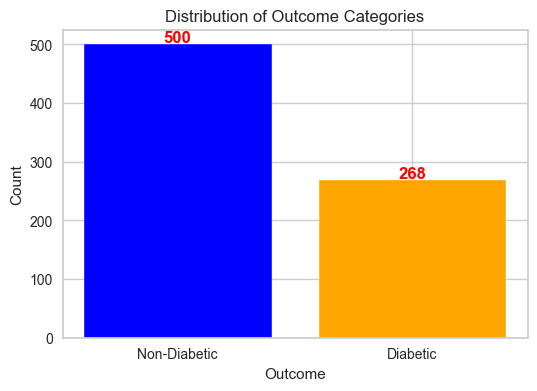
\includegraphics[width=0.55\textwidth]{images/outcome_distribution.png}
    \caption{Phân phối nhãn Outcome trong tập dữ liệu}
    \label{fig:outcome_dist}
\end{figure}

Hệ số tương quan Pearson giữa các đặc trưng đầu vào và nhãn mục tiêu được trực quan hóa ở Hình~\ref{fig:correlation_heatmap}. Kết quả tương quan cho thấy không có hiện tượng đa cộng tuyến quá mạnh giữa các biến độc lập.

\begin{figure}[H]
    \centering
    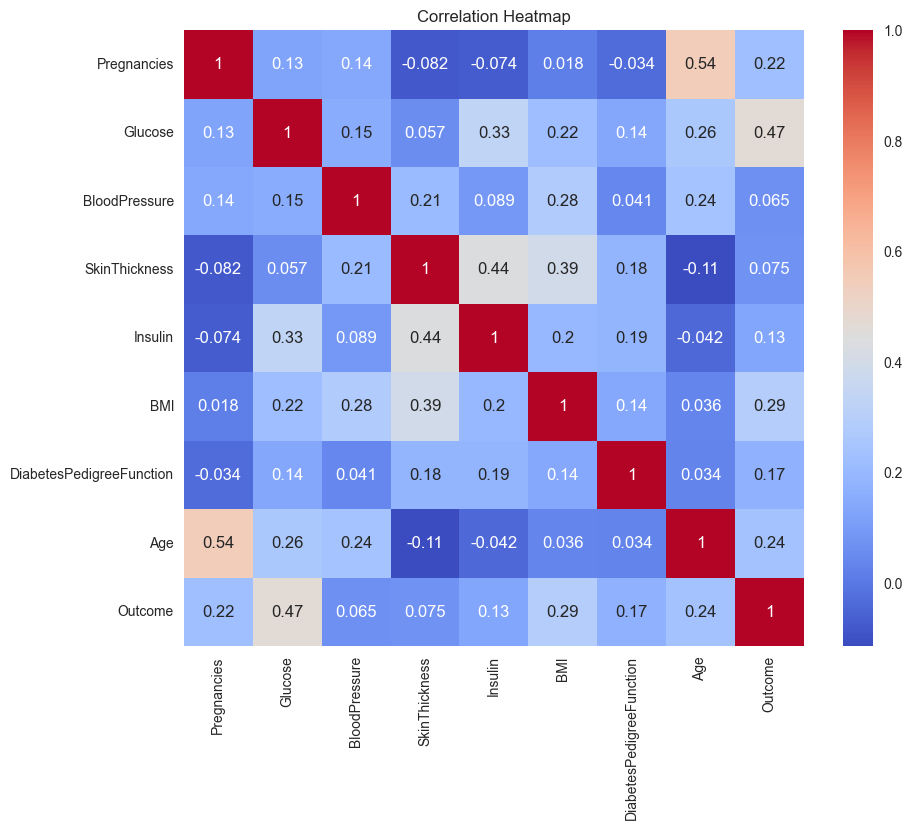
\includegraphics[width=0.7\textwidth]{images/correlation_heatmap.png}
    \caption{Ma trận tương quan Pearson giữa các thuộc tính}
    \label{fig:correlation_heatmap}
\end{figure}

\subsection{Chuẩn hóa dữ liệu bằng StandardScaler}
Vì thuật toán KNN sử dụng khoảng cách hình học giữa các điểm dữ liệu để phân lớp, việc các đặc trưng có thang đo chênh lệch lớn sẽ khiến các thuộc tính có khoảng giá trị rộng (như \texttt{Insulin} hay \texttt{Glucose}) lấn át hoàn toàn các thuộc tính có khoảng giá trị hẹp (như \texttt{DiabetesPedigreeFunction}). 

Chúng tôi sử dụng lớp chuẩn hóa \texttt{StandardScaler} để chuyển đổi các đặc trưng về dạng phân phối chuẩn hóa Z-score có trung bình bằng $0$ và phương sai bằng $1$:
\begin{equation}
    z = \frac{x - \mu}{\sigma}
\end{equation}
Trong đó $\mu$ là giá trị trung bình và $\sigma$ là độ lệch chuẩn của đặc trưng tương ứng trên tập huấn luyện. Sự phân bố của các thuộc tính sau khi chuẩn hóa được thể hiện trong Hình~\ref{fig:boxplot_after_scaler} và các khoảng giá trị cụ thể được trình bày ở Bảng~\ref{tab:scaled_ranges}.

\begin{figure}[H]
    \centering
    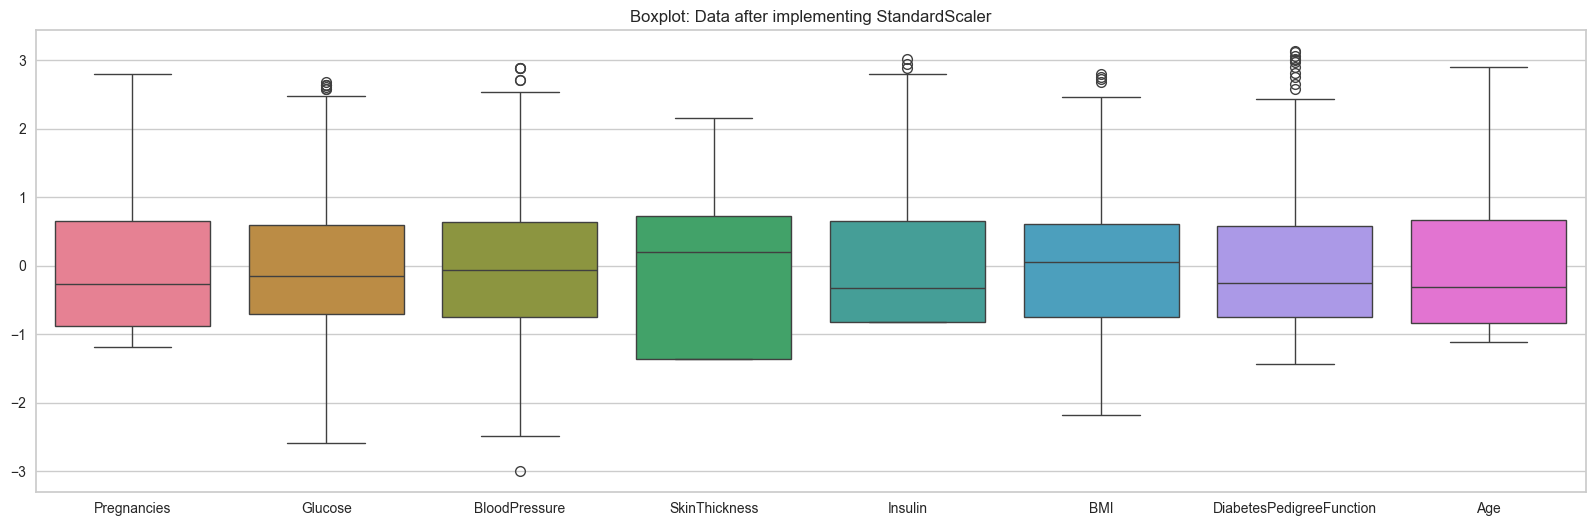
\includegraphics[width=0.9\textwidth]{images/boxplot_after_scaler.png}
    \caption{Biểu đồ Boxplot của dữ liệu sau khi áp dụng StandardScaler}
    \label{fig:boxplot_after_scaler}
\end{figure}

\begin{table}[H]
\centering
\caption{Khoảng giá trị của các đặc trưng sau chuẩn hóa}
\label{tab:scaled_ranges}
\begin{tabular}{lrrr}
\toprule
\textbf{Tên đặc trưng} & \textbf{Min (Scaled)} & \textbf{Max (Scaled)} & \textbf{Khoảng biến thiên} \\
\midrule
Pregnancies & -1.1896 & 2.7969 & 3.9865 \\
Glucose & -2.5937 & 2.6748 & 5.2685 \\
BloodPressure & -3.0017 & 2.8775 & 5.8792 \\
SkinThickness & -1.3594 & 2.1591 & 3.5185 \\
Insulin & -0.8300 & 3.0125 & 3.8425 \\
BMI & -2.1750 & 2.7929 & 4.9679 \\
DiabetesPedigreeFunction & -1.4335 & 3.1282 & 4.5616 \\
Age & -1.1112 & 2.9032 & 4.0144 \\
\bottomrule
\end{tabular}
\end{table}

\section{Tìm kiếm siêu tham số và Kết quả Baseline KNN}
Tập dữ liệu sau khi loại bỏ ngoại lai được phân chia theo tỷ lệ $70/30$ độc lập: tập huấn luyện gồm $447$ mẫu và tập kiểm thử gồm $192$ mẫu.

\subsection{Tìm kiếm siêu tham số $k$ tối ưu bằng phương pháp Hold-out}
Để tìm ra số lân cận $k$ phù hợp nhất mà không gây rò rỉ thông tin từ tập kiểm thử, tập huấn luyện được chia tiếp thành tập huấn luyện con (\texttt{X\_train\_sub} - $80\%$, $357$ mẫu) và tập kiểm định (\texttt{X\_val} - $20\%$, $90$ mẫu). Chúng tôi tiến hành huấn luyện KNN với các giá trị $k$ từ $1$ đến $29$ và đánh giá độ chính xác trên tập kiểm định \texttt{X\_val}.

\begin{figure}[H]
    \centering
    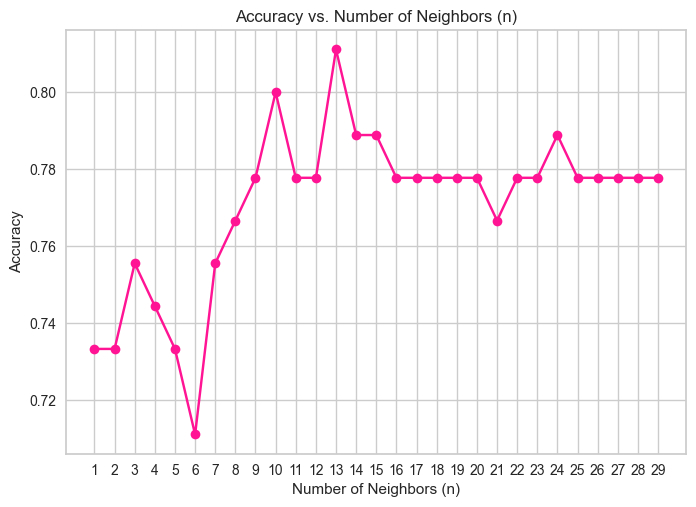
\includegraphics[width=0.7\textwidth]{images/tuning_accuracy_vs_n.png}
    \caption{Độ chính xác của mô hình tương ứng với các giá trị $k$}
    \label{fig:accuracy_k}
\end{figure}

Dựa trên kết quả ở Hình~\ref{fig:accuracy_k}, độ chính xác trên tập validation đạt mức cao nhất và có xu hướng ổn định tại \textbf{$k = 13$} (đạt độ chính xác $78.89\%$). Do đó, siêu tham số $k = 13$ được lựa chọn để huấn luyện mô hình Baseline KNN.

\subsection{Đánh giá kết quả mô hình Baseline trên tập kiểm thử}
Mô hình KNN baseline với tham số $k = 13$ sử dụng toàn bộ $8$ đặc trưng được huấn luyện trên tập huấn luyện đầy đủ và đánh giá hiệu năng trên tập kiểm thử độc lập \texttt{X\_test}.

Độ chính xác tổng thể (Accuracy) của mô hình đạt \textbf{$81.25\%$}. Báo cáo phân loại chi tiết (Classification Report) được thể hiện trong Bảng~\ref{tab:classification_baseline}.

\begin{table}[H]
\centering
\caption{Hiệu năng chi tiết của mô hình Baseline KNN ($k=13$)}
\label{tab:classification_baseline}
\begin{tabular}{ccccc}
\toprule
\textbf{Lớp} & \textbf{Precision} & \textbf{Recall} & \textbf{F1-Score} & \textbf{Support} \\
\midrule
0 (Không tiểu đường) & 0.8165 & 0.9485 & 0.8776 & 136 \\
1 (Mắc tiểu đường) & 0.7941 & 0.4821 & 0.6000 & 56 \\
\midrule
\textbf{Accuracy} & & & \textbf{0.8125} & 192 \\
\textbf{Macro Average} & 0.8053 & 0.7153 & 0.7388 & 192 \\
\textbf{Weighted Average} & 0.8099 & 0.8125 & 0.7966 & 192 \\
\bottomrule
\end{tabular}
\end{table}

Ma trận nhầm lẫn của mô hình Baseline KNN được mô tả trong Hình~\ref{fig:confusion_baseline}:

\begin{figure}[H]
    \centering
    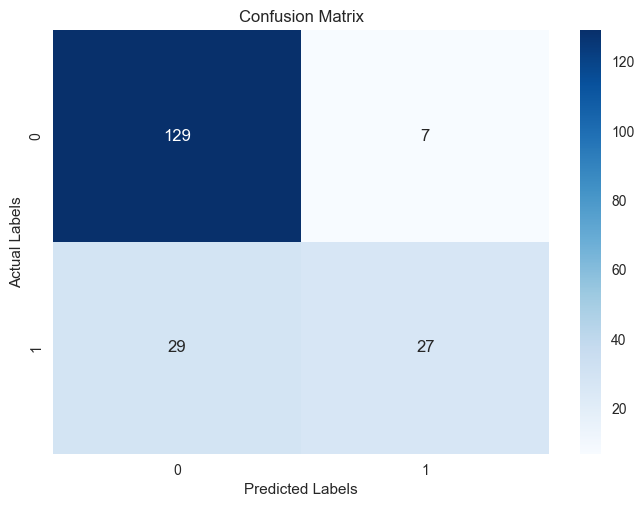
\includegraphics[width=0.55\textwidth]{images/confusion_matrix_baseline.png}
    \caption{Ma trận nhầm lẫn của mô hình Baseline KNN với $k=13$}
    \label{fig:confusion_baseline}
\end{figure}

\subsection{Nhận xét kết quả Baseline}
Mặc dù mô hình Baseline KNN đạt độ chính xác chung $81.25\%$, nhưng khả năng dự đoán bệnh nhân mắc tiểu đường (lớp 1) còn rất hạn chế:
\begin{itemize}
    \item Độ nhạy (Recall) của lớp 1 chỉ đạt $48.21\%$, nghĩa là mô hình đã bỏ sót tới $29$ bệnh nhân mắc bệnh tiểu đường trên thực tế (gán nhãn nhầm thành khỏe mạnh).
    \item F1-Score của lớp 1 cũng chỉ đạt $0.6000$.
\end{itemize}
Nguyên nhân là do việc tính khoảng cách hình học của KNN bao gồm cả những đặc trưng kém quan trọng hoặc gây nhiễu, làm mờ đi thông tin cốt lõi của các đặc trưng chính. Do đó, việc tối ưu hóa lựa chọn đặc trưng là cực kỳ cần thiết.

% ==========================================
% CHƯƠNG III: TỐI ƯU HÓA ĐẶC TRƯNG BẰNG PSO
% ==========================================
\chapter{Tối ưu hóa đặc trưng bằng Particle Swarm Optimization}

\section{Lý thuyết Thuật toán tối ưu hóa bầy đàn nhị phân (Binary PSO)}
Lựa chọn đặc trưng (Feature Selection) là một bài toán tối ưu hóa tổ hợp rời rạc nhằm tìm kiếm một tập con các thuộc tính từ tập ban đầu sao cho hiệu năng dự đoán của mô hình được cải thiện nhiều nhất. Với $d$ đặc trưng ban đầu, không gian tìm kiếm chứa $2^d$ tập con khả thi. 

Thuật toán Tối ưu hóa Bầy đàn nhị phân (Binary Particle Swarm Optimization - BPSO), được đề xuất bởi Kennedy và Eberhart, là một thuật toán tối ưu hóa metaheuristic mô phỏng hành vi di chuyển bầy đàn của chim hoặc cá trong không gian rời rạc để giải quyết bài toán này.

\subsection{Mô hình hóa hạt trong không gian nhị phân}
Trong BPSO, mỗi hạt (particle) $i$ đại diện cho một phương án lựa chọn đặc trưng, được xác định bởi:
\begin{itemize}
    \item \textbf{Vị trí nhị phân} $x_i^t = (x_{i1}^t, x_{i2}^t, \dots, x_{id}^t) \in \{0, 1\}^d$, trong đó $x_{ij}^t = 1$ biểu thị đặc trưng thứ $j$ được lựa chọn và $x_{ij}^t = 0$ nghĩa là đặc trưng thứ $j$ bị loại bỏ.
    \item \textbf{Vận tốc liên tục} $v_i^t = (v_{i1}^t, v_{i2}^t, \dots, v_{id}^t) \in \mathbb{R}^d$, đại diện cho xác suất thay đổi trạng thái nhị phân của các chiều tương ứng.
    \item \textbf{Vị trí tốt nhất cá nhân} $pbest_i^t$: Vị trí có độ thích nghi tốt nhất mà hạt $i$ từng đi qua tính đến thời điểm $t$.
    \item \textbf{Vị trí tốt nhất bầy đàn} $gbest^t$: Vị trí tốt nhất trong số toàn bộ các $pbest_i^t$ của cả bầy đàn tính đến thời điểm $t$.
\end{itemize}

\subsection{Cơ chế cập nhật vận tốc và vị trí}
Tại mỗi thế hệ hay bước lặp $t+1$, vận tốc liên tục của hạt $i$ trên chiều đặc trưng $j$ được cập nhật theo công thức động lực học:
\begin{equation}
    v_{ij}^{t+1} = w \cdot v_{ij}^t + c_1 r_1 (pbest_{ij} - x_{ij}^t) + c_2 r_2 (gbest_j - x_{ij}^t)
\end{equation}
Trong đó:
\begin{itemize}
    \item $w$: Trọng số quán tính (inertia weight), kiểm soát khả năng khám phá không gian mới của hạt.
    \item $c_1, c_2$: Các hệ số nhận thức cá nhân và hệ số xã hội.
    \item $r_1, r_2$: Các số ngẫu nhiên phân phối đều độc lập trong khoảng $[0, 1]$.
\end{itemize}

Để đảm bảo thuật toán không bị phân kỳ, vận tốc của hạt được khống chế trong khoảng giới hạn $[-V_{\max}, V_{\max}]$:
\begin{equation}
    v_{ij}^{t+1} = \max(-V_{\max}, \min(V_{\max}, v_{ij}^{t+1}))
\end{equation}
Trong thực nghiệm này, giá trị vận tốc giới hạn được đặt là $V_{\max} = 6.0$.

Vị trí nhị phân $x_{ij}^{t+1}$ được cập nhật thông qua hàm truyền dạng Sigmoid ($S$-shape transfer function) để chuyển đổi vận tốc thực sang xác suất nhị phân:
\begin{equation}
    S(v_{ij}^{t+1}) = \frac{1}{1 + e^{-v_{ij}^{t+1}}}
\end{equation}
Vị trí mới được cập nhật theo xác suất này bằng quy tắc:
\begin{equation}
    x_{ij}^{t+1} = \begin{cases}
        1 & \text{nếu } \text{rand}() < S(v_{ij}^{t+1}) \\
        0 & \text{ngược lại}
    \end{cases}
\end{equation}
Trong đó $\text{rand}()$ là một số ngẫu nhiên phân phối đều trong khoảng $[0, 1]$. Trong trường hợp một hạt cập nhật ra tất cả vị trí bằng 0 ($x_{ij} = 0, \forall j$), thuật toán sẽ chọn ngẫu nhiên một đặc trưng bất kỳ gán bằng 1 để đảm bảo mô hình KNN luôn nhận tối thiểu một đặc trưng để tính khoảng cách.

\section{Thiết kế Hàm thích nghi (Fitness Function)}
Hàm thích nghi (Fitness Function) đóng vai trò quyết định hướng hội tụ của bầy đàn hạt. Mục tiêu của bài toán là tối đa hóa độ chính xác phân loại của KNN, đồng thời tối thiểu hóa số lượng đặc trưng được lựa chọn để mô hình gọn nhẹ nhất.

Hàm thích nghi được thiết kế dưới dạng hàm đa mục tiêu tuyến tính kết hợp thành phần phạt số lượng đặc trưng:
\begin{equation}
    \text{Fitness} = \alpha \cdot \text{Accuracy}_{\text{val}} + (1 - \alpha) \cdot \left(1 - \frac{N_{\text{selected}}}{N_{\text{total}}}\right)
\end{equation}
Trong đó:
\begin{itemize}
    \item $\text{Accuracy}_{\text{val}}$: Độ chính xác của mô hình KNN trên tập kiểm định \texttt{X\_val}.
    \item $N_{\text{selected}}$: Số lượng đặc trưng được chọn trong cấu hình hiện tại (số bit 1 trong vector $x_i$).
    \item $N_{\text{total}}$: Tổng số đặc trưng ban đầu ($N_{\text{total}} = 8$).
    \item $\alpha$: Trọng số kiểm soát sự ưu tiên. Do độ chính xác phân loại y tế là mục tiêu tối thượng, chúng tôi thiết lập $\alpha = 0.99$. Thành phần phạt nhỏ $(1-\alpha) = 0.01$ đóng vai trò giải quyết tranh chấp nhãn: nếu hai tập đặc trưng khác nhau mang lại cùng một độ chính xác, tập đặc trưng ít chiều hơn sẽ có độ thích nghi cao hơn.
\end{itemize}

\section{Kết quả tối ưu hóa đặc trưng và So sánh hiệu năng}
Thuật toán BPSO được thực thi với kích thước bầy đàn $N = 15$ hạt và số lượng vòng lặp tối đa là $30$. Mô hình phân lớp cơ sở được sử dụng là KNN cài đặt từ đầu với tham số $k = 13$ tối ưu. Toàn bộ tập kiểm thử \texttt{X\_test} được giữ độc lập tuyệt đối để tránh rò rỉ dữ liệu trong quá trình tối ưu.

\subsection{Quá trình tối ưu hóa đặc trưng của PSO}
Tiến trình tìm kiếm của bầy đàn qua các thế hệ được ghi nhận như sau:
\begin{itemize}
    \item \textbf{Vòng lặp 1:} Thu được tập 5 đặc trưng có độ chính xác kiểm định đạt $0.7556$.
    \item \textbf{Vòng lặp 2:} Thu được tập 4 đặc trưng có độ chính xác kiểm định đạt $0.7889$.
    \item \textbf{Vòng lặp 6 đến 30:} Thuật toán hội tụ và tìm ra tập chỉ gồm \textbf{3 đặc trưng} tối ưu nhất mang lại độ chính xác kiểm định cao nhất là \textbf{$0.8111$}.
\end{itemize}

Ba đặc trưng y tế quan trọng nhất được thuật toán PSO lựa chọn bao gồm:
\begin{enumerate}
    \item \textbf{Glucose}: Nồng độ đường huyết.
    \item \textbf{DiabetesPedigreeFunction}: Chỉ số phả hệ di truyền tiểu đường.
    \item \textbf{Age}: Độ tuổi.
\end{enumerate}
Năm đặc trưng còn lại (\texttt{Pregnancies}, \texttt{BloodPressure}, \texttt{SkinThickness}, \texttt{Insulin}, \texttt{BMI}) đã bị thuật toán PSO loại bỏ do không đóng góp nhiều thông tin hoặc gây nhiễu cho thuật toán phân lớp KNN (giảm $62.5\%$ số lượng đặc trưng đầu vào).

\subsection{So sánh hiệu năng giữa Baseline KNN và PSO-KNN}
Mô hình KNN với tham số $k=13$ chỉ sử dụng 3 đặc trưng tối ưu đã chọn được huấn luyện lại trên toàn bộ tập huấn luyện và dự đoán trên tập kiểm thử độc lập \texttt{X\_test}.

Độ chính xác tổng thể tăng lên đạt \textbf{$82.81\%$} (tăng $1.56\%$ so với baseline $81.25\%$). Bảng~\ref{tab:comparison_metrics} trình bày sự đối sánh chi tiết hiệu năng giữa mô hình Baseline KNN sử dụng đầy đủ 8 đặc trưng và mô hình PSO-KNN sử dụng 3 đặc trưng tối ưu.

\begin{table}[H]
\centering
\caption{So sánh hiệu năng của Baseline KNN và PSO-KNN trên tập kiểm thử}
\label{tab:comparison_metrics}
\begin{tabular}{lcccccc}
\toprule
\textbf{Mô hình} & \textbf{Số đặc trưng} & \textbf{Lớp} & \textbf{Precision} & \textbf{Recall} & \textbf{F1-Score} & \textbf{Accuracy} \\
\midrule
Baseline KNN & 8 & Lớp 0 & 0.8165 & \textbf{0.9485} & 0.8776 & 0.8125 \\
             &   & Lớp 1 & \textbf{0.7941} & 0.4821 & 0.6000 & \\
\midrule
\textbf{PSO-KNN} & \textbf{3} & Lớp 0 & \textbf{0.8411} & 0.9338 & \textbf{0.8850} & \textbf{0.8281} \\
                 &   & Lớp 1 & 0.7805 & \textbf{0.5714} & \textbf{0.6598} & \\
\bottomrule
\end{tabular}
\end{table}

Hình~\ref{fig:confusion_comparison} trình bày so sánh trực quan Ma trận nhầm lẫn của mô hình Baseline KNN và mô hình cải tiến PSO-KNN trên tập kiểm thử.

\begin{figure}[H]
    \centering
    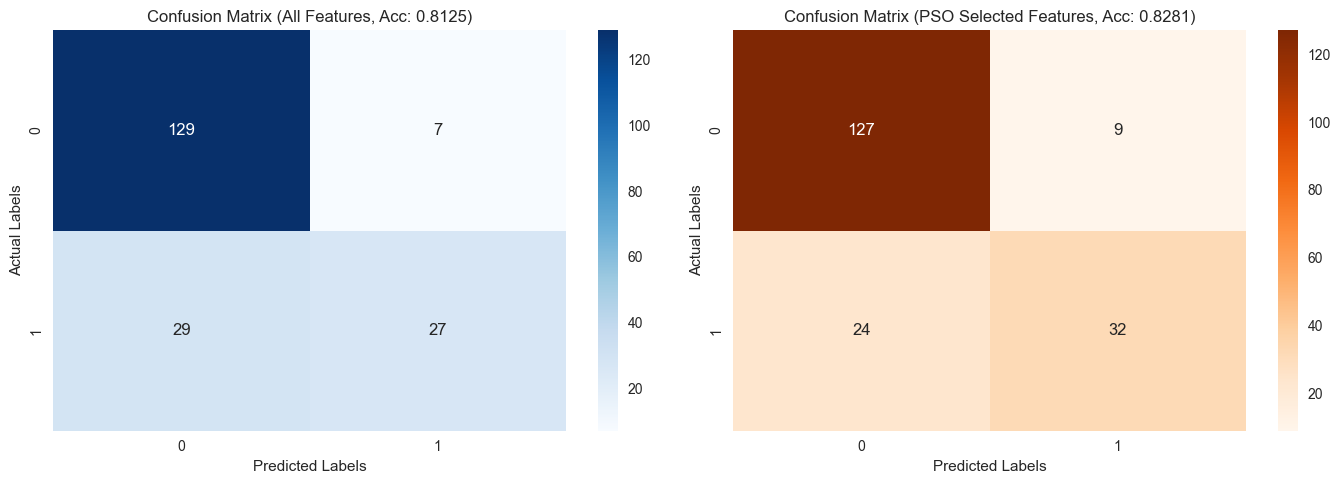
\includegraphics[width=0.95\textwidth]{images/confusion_matrix_comparison.png}
    \caption{So sánh ma trận nhầm lẫn giữa Baseline KNN và PSO-KNN}
    \label{fig:confusion_comparison}
\end{figure}

\subsection{Nhận xét sự cải tiến}
Việc áp dụng giải thuật tối ưu hóa đặc trưng BPSO mang lại hiệu quả vượt trội cho mô hình phân lớp KNN:
\begin{enumerate}
    \item \textbf{Cải thiện mạnh độ nhạy (Recall) của lớp mắc bệnh (Lớp 1):} Tăng đáng kể từ $48.21\%$ lên $57.14\%$ (tăng $8.93\%$). Mô hình PSO-KNN đã phát hiện chính xác thêm $5$ bệnh nhân mắc tiểu đường thực tế bị mô hình Baseline bỏ sót. Điều này cực kỳ có ý nghĩa trong bài toán sàng lọc y tế nhằm tránh bỏ sót người bệnh.
    \item \textbf{F1-Score tăng ở cả hai nhóm phân lớp:} Đặc biệt F1-Score của lớp bệnh nhân mắc tiểu đường tăng từ $0.6000$ lên $0.6598$.
    \item \textbf{Giảm độ phức tạp tính toán:} Số lượng đặc trưng giảm $62.5\%$ giúp không gian tính toán khoảng cách của KNN thu gọn đáng kể, giảm thời gian xử lý và lưu trữ của hệ thống.
\end{enumerate}

Hình~\ref{fig:decision_boundary} minh họa ranh giới quyết định (Decision Boundary) của mô hình tối ưu KNN với $k = 13$ dựa trên không gian đặc trưng đã được thu gọn.

\begin{figure}[H]
    \centering
    
\includegraphics[width=0.75\textwidth]{images/decision_boundary_k13.png}
    \caption{Ranh giới quyết định phân lớp của mô hình PSO-KNN với $k=13$}
    \label{fig:decision_boundary}
\end{figure}

Ranh giới phân lớp có xu hướng trơn tru, phân định rõ ràng các vùng tập trung mẫu mà không xuất hiện các phân vùng nhỏ vụn phân tán, chứng minh mô hình hoạt động ổn định và có khả năng tổng quát hóa tốt trên dữ liệu mới thực tế.

\newpage
\begin{thebibliography}{99}

\bibitem{kennedy1995}
J. Kennedy and R. Eberhart, "Particle swarm optimization," in \textit{Proceedings of ICNN'95 - International Conference on Neural Networks}, vol. 4, pp. 1942-1948, 1995.

\bibitem{shi1998}
Y. Shi and R. Eberhart, "A modified particle swarm optimizer," in \textit{1998 IEEE International Conference on Evolutionary Computation Proceedings}, pp. 69-73, 1998.

\bibitem{clerc2002}
M. Clerc and J. Kennedy, "The particle swarm - explosion, stability, and convergence in a multidimensional complex space," \textit{IEEE Transactions on Evolutionary Computation}, vol. 6, no. 1, pp. 58-73, 2002.

\end{thebibliography}

\end{document}
